\documentclass[a4paper,10pt]{article}
\usepackage{mathptmx}

\usepackage{tabularx} % extra features for tabular environment
\usepackage{amsmath}  % improve math presentation
\usepackage{float}
% \usepackage{pdfpages}


\usepackage{graphicx} % takes care of graphic including machinery
\graphicspath{ {./figures/} }
%\usepackage[margin=1in,letterpaper]{geometry} % decreases margins
%\usepackage{cite} % takes care of citations
\usepackage[final]{hyperref} % adds hyper links inside the generated pdf file
\hypersetup{
	colorlinks=true,       % false: boxed links; true: colored links
	linkcolor=blue,        % color of internal links
	citecolor=blue,        % color of links to bibliography
	filecolor=magenta,     % color of file links
	urlcolor =blue         
}
\usepackage[margin = 1in,headsep=0.5cm,headheight=2cm,letterpaper]{geometry} 

\usepackage{fancyhdr}
\pagestyle{fancy}
\lhead{Student 1 : Ahmet Akman 2442366 \\ Student 2: Kaan Demirkoparan }
\rhead{Date: \today \\ Group: Friday Morning - 6} 
%\cfoot{center of the footer!}
%\renewcommand{\headrulewidth}{0.1pt}


\begin{document}
%\thispagestyle{empty}

\title{  Fall 2022 EE Project Work  \protect\\ Preliminary Report}
\author{ Ahmet Akman 2442366 \protect\\ Kaan Demirkoparan}
\date{}
\maketitle
%\tableofcontents
%\begin{abstract}
%abstract
%\end{abstract}
\section{Introduction}
In this document, the Preliminary report of the term project of the EE214 course will be presented. 
\section{General Structure and Design Philisophy}
\begin{figure}[h]
    \centering
    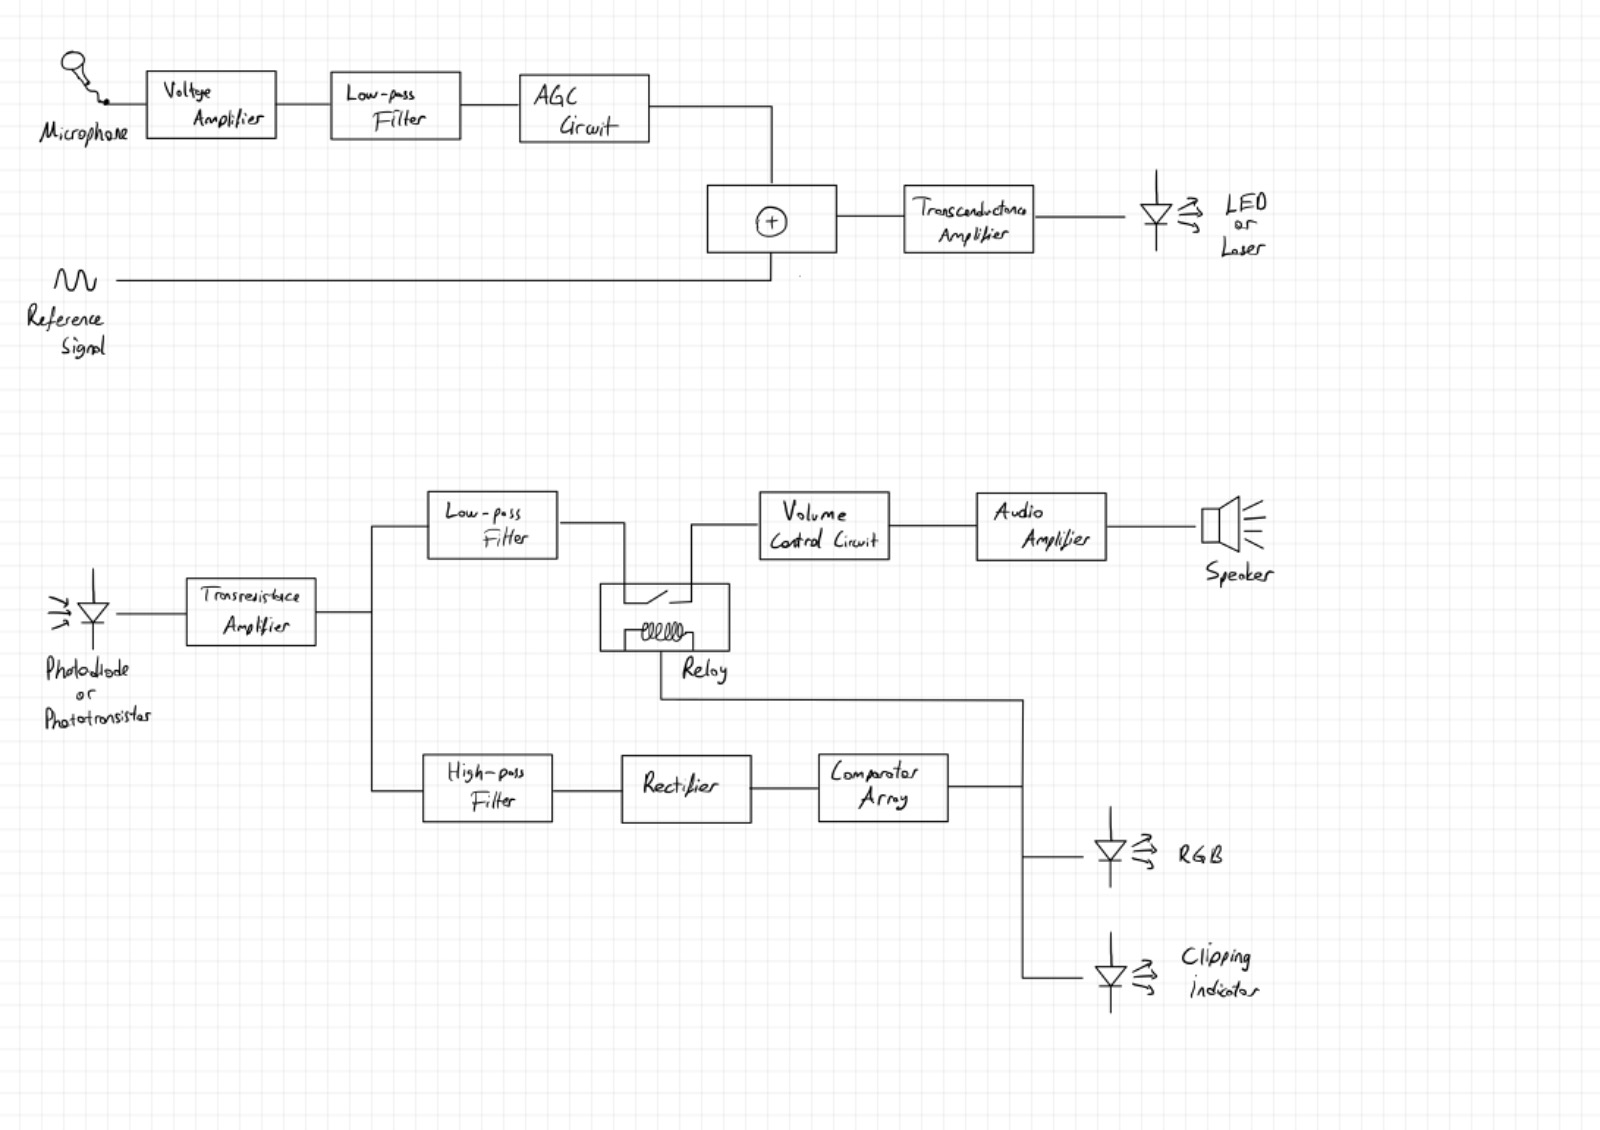
\includegraphics[width = 1\textwidth]{general_structure.jpeg}
    \caption{General Structure}
\end{figure} 
Deneme
Deneme 123 Deneme 123

xyz

\section{Transmitter Side}
\subsection{Input and Early Stage Amplification}
\subsection{Automatic Gain Control}
\subsection{Light Transmitter}
\section{Receiver Side}
\subsection{Light Receiver}
\subsection{Demodulation and Speaker Side}
At the beggining of this stage a simple op-amp buffer will planned to be used in order to prevent distorion while using the same signal as input for two stages in parallel. For the demodulation of the input signal (a.k.a. filtering out the carrier high frequency components), a low pass filter will planned to be used. There are two basic  option for low pass filtering. First one is passive RC/RL filters. They use few components but have no gain and there is no tunability. Second one is active opamp-filters. Even though they seem more complicated one can have gain and a more flexible design. The required low pass charachteristic is given in Figure \ref*{low_pass_plot}
\begin{figure}[H]
    \centering
    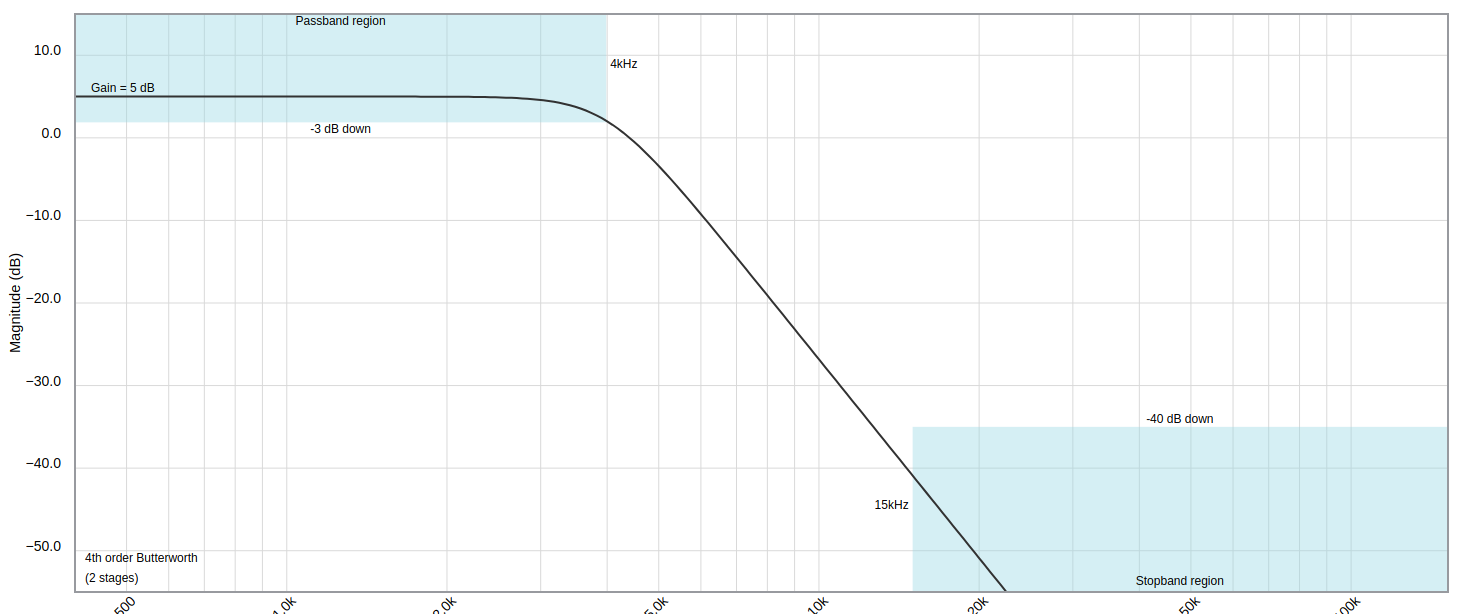
\includegraphics[width = 0.75\textwidth]{active_low_pass.png}
    \caption{Low pass filter frequency response}
    \label{low_pass_plot}    
\end{figure} 
Because of the aforementioned advantages our design decision is using active two stage low pass filter with butterworth response. A premature design is given in Figure \ref*{low_pass_sch}
\begin{figure}[H]
    \centering
    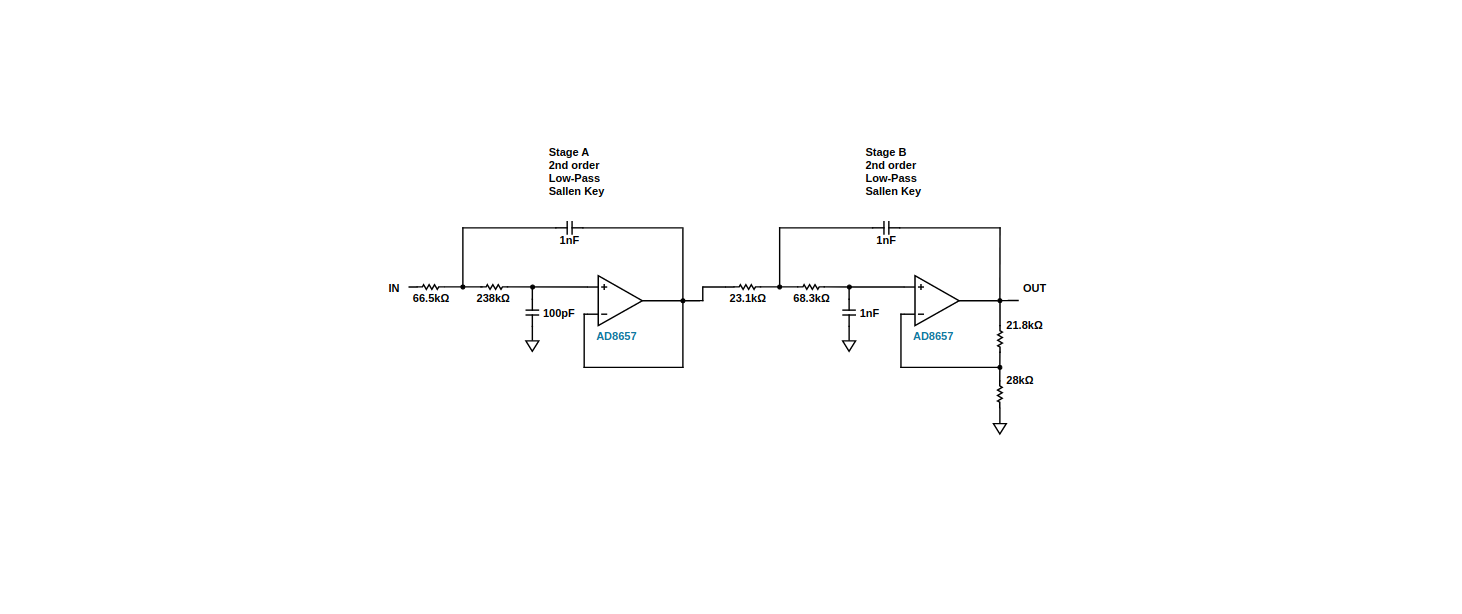
\includegraphics[width = 0.75\textwidth]{active_low_pass_circuit.png}
    \caption{Active low pass filter design}
    \label{low_pass_sch}    
\end{figure} 
%LOW SİGNAL SWİTCH PART WILL BE ADDED
Since, now we have a nice signal that carries the information needed, we should amplify it properly in order to drive the speaker. For the design purpose we assume our speaker is 16\(\Omega\) ,and our design constraint is that our speaker will operate with 1W power.
   
\subsection{Signal Quality Indication}

\section{Conclusion}
In this document, the Preliminary report of the term project of the EE313 course is presented. 

\end{document}

%%%%%%%%%%%%%%%%%%%%%%   EXAMPLE TABLE   %%%%%%%%%%%%%%%%%%%%%%%%%%%%%%%%
\begin{table}[H]
\begin{center}
    \caption{Resistance reading by color code convention.}
    \vspace{2mm}
    \begin{tabular}{||c | c | c||} 
        \hline
        Color Order & Value & Tolerance \\ [0.5ex] 
        \hline\hline
        Brown / Black / Red / Gold & 1k\( \Omega \) & \( \% \) 5  \\ 
        \hline
        Yellow / Violet / Red / Gold & 4.7k\( \Omega \) & \( \% \) 5   \\
        \hline
        Brown / Grey / Orange / Gold & 18k\( \Omega \) & \( \% \) 5  \\ [1ex] 
        \hline
    \end{tabular}
\end{center}
\end{table}


%%%%%%%%%%%%%%%%%%%%%%   EXAMPLE IMAGE   %%%%%%%%%%%%%%%%%%%%%%%%%%%%%%%%
\begin{figure}[H]
\centering
\includegraphics[width = 0.75\textwidth]{5.png}
\caption{Circuit schematic for the step 5}
\end{figure} 

%%%%%%%%%%%%%%%%%%%%%%   EXAMPLE IMAGE FROM PDF   %%%%%%%%%%%%%%%%%%%%%%%%%%%%%%%%
\begin{figure}[H] \centering{
	\includegraphics[scale=0.25]{2a_plot.pdf}}
	\caption{Experiment 2}
\end{figure}
%%%%%%%%%%%%%%%% Deneme Push